\label{chp:benchmark}
\section{Implementation}

All algorithms were implemented using C++20 for an open-source KOALA NetworKit library \cite{koala-networkit}. 

\subsection{KOALA NetworKit}

Short descriptions found in the README file in the cited repository accurately describe the building blocks of the project.

\begin{itemize}
    \item \textbf{NetworKit} is an open-source general-purpose network analysis and graph mining library written in C++. Graphs are represented in a very compact form while the efficiency of changes to their structure, such as node and edge additions or deletions, is preserved. The memory-saving design is related to the main aim of the library: the analysis of large-scale random graphs and real-world networks.
    \item \textbf{KOALA} is an open-source library of C++ templates, developed at the Gdansk University of Technology, Department of Algorithms and System Modeling. Its main part consists of an implementation of a broad set of procedures in the fields of algorithmic graph theory and network problems in discrete optimization.
\end{itemize}

The project also invokes functions of \textbf{Boost} library and uses \textbf{GoogleTest} for unit testing. Additionally, \textbf{nauty} package is used for generating and reading random test graphs.

\subsection{Implementation details and expectations}

Major changes were added in the following files:
\begin{itemize}  [noitemsep]
    \item \texttt{include/mis/IndependentSet.hpp} -- header file with all necessary function declarations
    \item \texttt{cpp/mis/IndependentSet.cpp} -- source file with helper functions for all algorithms as well as the implementation of \textsc{MisNaive}
    \item \texttt{cpp/mis/ExactRecursiveIndependentSet.cpp} -- source file with implementation of all recursive algorithms
    \item \texttt{test/testIndependentSet.cpp} -- simple GoogleTest tests added mainly to improve user understanding and experience as well as provide some basic testing
    \item \texttt{benchmark/benchmarkIndependentSet.cpp} -- an independent program that allows for extensive benchmark testing of all algorithms using graphs generated from \cite{benchmark}
\end{itemize}

Almost all algorithms except \textsc{MisNaive} intensively use recursive calls. For that reason, we decided to avoid copying \texttt{NetworKit::graph} and instead, we modify it before a recursive call and revert changes after. Generally speaking, \texttt{Networkit::graph} structure does not perform well in situations where the graph is heavily modified. Algorithms also can not take full advantage of a reduced size of a problem because of how NetworKit is implemented. There is no efficient way to resize a graph (and resize back) for smaller subgraphs of the original problem.

For these reasons, it is worth noting that we can expect high overhead for \textsc{MisFolding} algorithm since it modifies graphs the most. Besides that, a polynomial factor of complexity, which was completely ignored in the article, for \textsc{MisFolding} is quite high. It is to be expected that \textsc{Mis2} to perform the best for relatively small graphs but hopefully will be outperformed by \textsc{MisFolding} for larger ones. \textsc{Mis3}, \textsc{Mis4}, \textsc{Mis5} will likely perform almost the same. \textsc{Mis1} will probably be the second slowest after \textsc{MisNaive}. \textsc{MisNaive} will even have to be skipped in computationally demanding benchmark tests due to unworldly long execution times but it should be the fastest for very small graphs.

\subsection{Correctness}

Each of the algorithm solutions is verified whether it is an independent set. It means that for every returned solution $I$ for test graph $G = (V, E)$ we make sure that there are no vertices $u,v\in I$ such that there is an edge $\{u,v\} \in E$.

Additionally, we check whether all algorithms for the same test, return the same maximum independent set size. The indispensable algorithm here is \textsc{MisNaive} as it is pretty much impossible to be incorrect due to its simplicity.

\clearpage

\section{Benchmark results}

\begin{figure}[H]
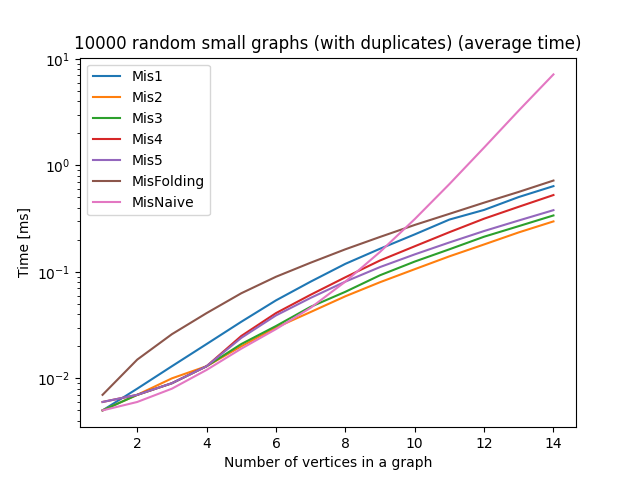
\includegraphics[width=\textwidth]{4_benchmark/plots/small.png}
\centering
\end{figure}

\begin{figure}[H]
\vspace{-1cm}
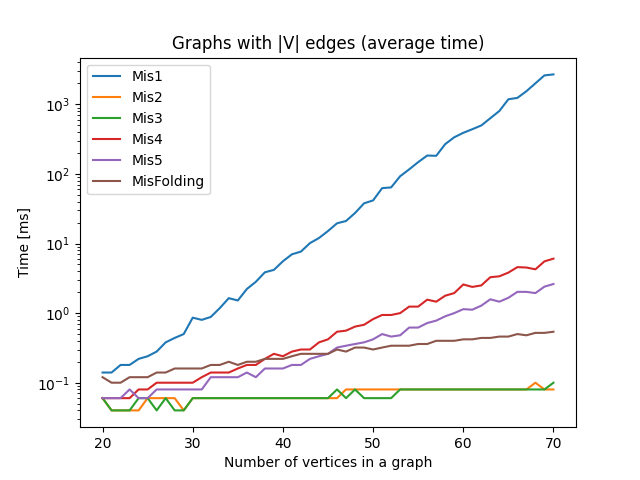
\includegraphics[width=\textwidth]{4_benchmark/plots/1n.png}
\centering
\end{figure}

\begin{figure}[H]
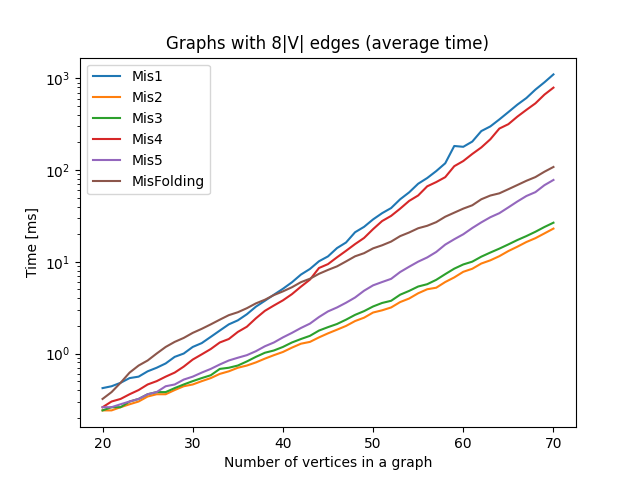
\includegraphics[width=\textwidth]{4_benchmark/plots/8n.png}
\centering
\end{figure}

\begin{figure}[H]
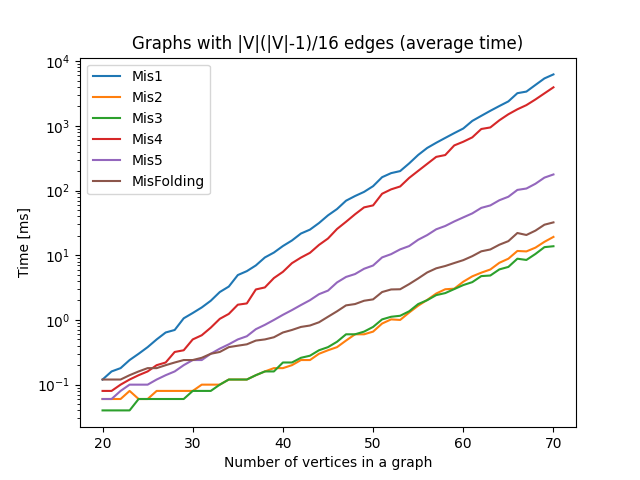
\includegraphics[width=\textwidth]{4_benchmark/plots/0.0625n2.png}
\centering
\end{figure}

\begin{figure}[H]
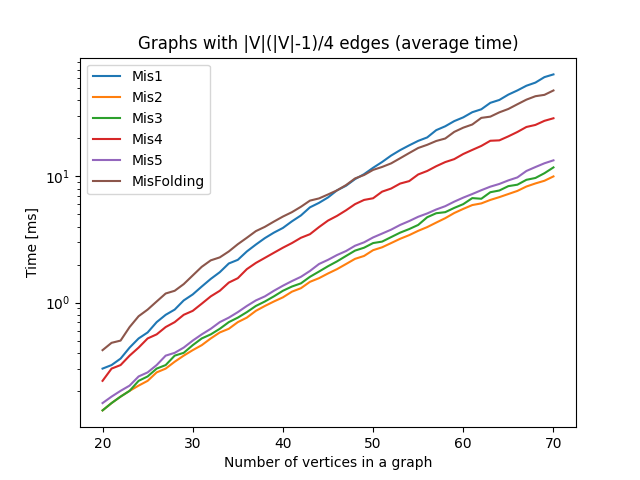
\includegraphics[width=\textwidth]{4_benchmark/plots/0.25n2.png}
\centering
\end{figure}

\begin{figure}[H]
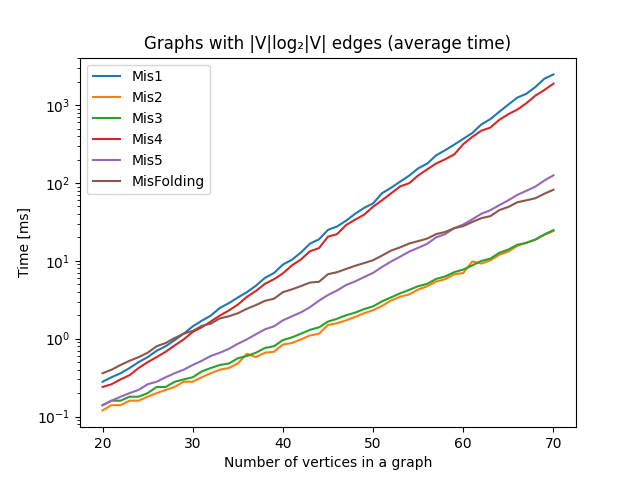
\includegraphics[width=\textwidth]{4_benchmark/plots/1nlogn.png}
\centering
\end{figure}

\begin{figure}[H]
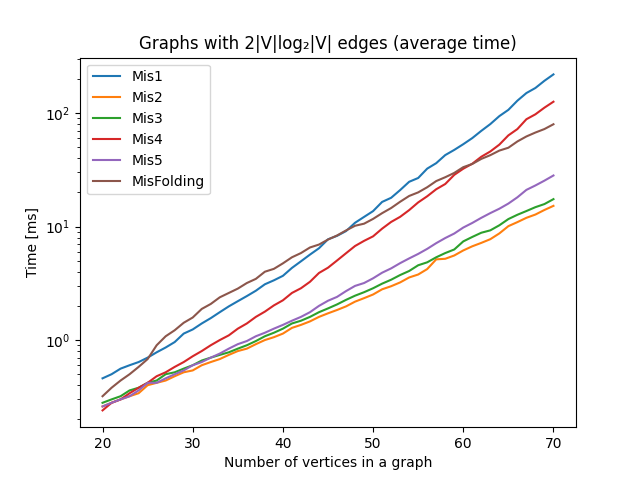
\includegraphics[width=\textwidth]{4_benchmark/plots/2nlogn.png}
\centering
\end{figure}

\begin{figure}[H]
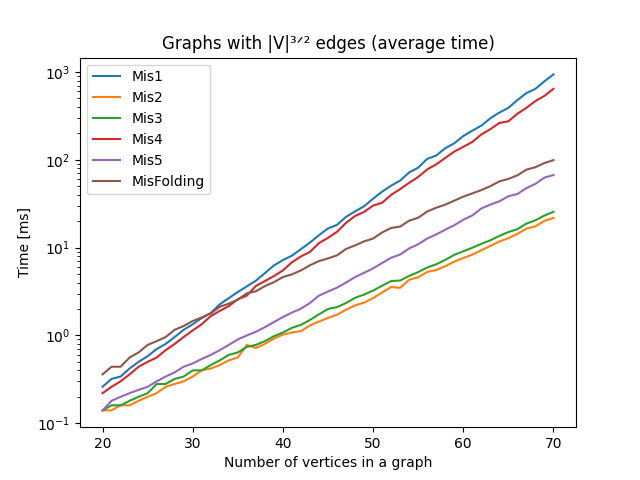
\includegraphics[width=\textwidth]{4_benchmark/plots/1n32.png}
\centering
\end{figure}

\begin{figure}[H]
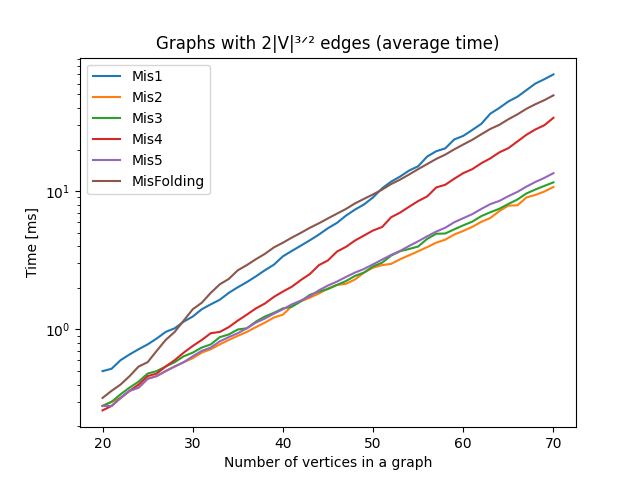
\includegraphics[width=\textwidth]{4_benchmark/plots/2n32.png}
\centering
\end{figure}

\begin{figure}[H]
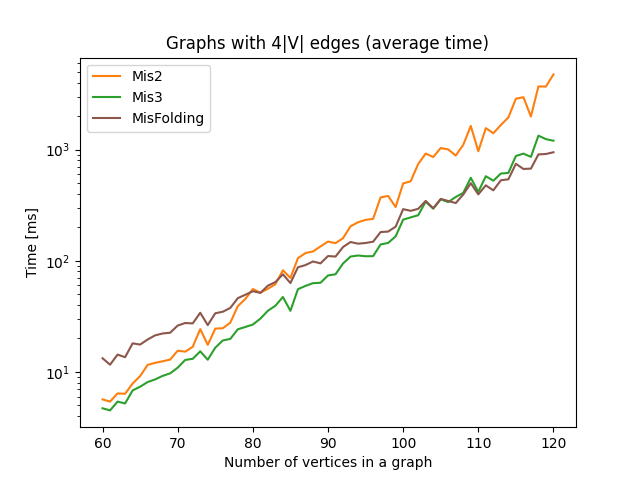
\includegraphics[width=\textwidth]{4_benchmark/plots/big4n.png}
\centering
\end{figure}

\begin{figure}[H]
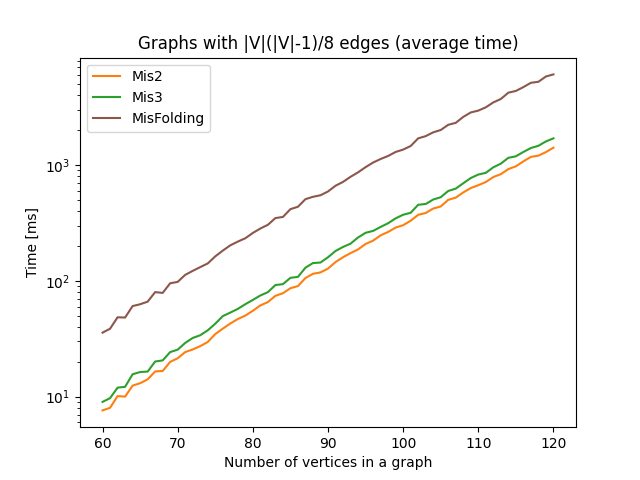
\includegraphics[width=\textwidth]{4_benchmark/plots/bign2.png}
\centering
\end{figure}

\begin{figure}[H]
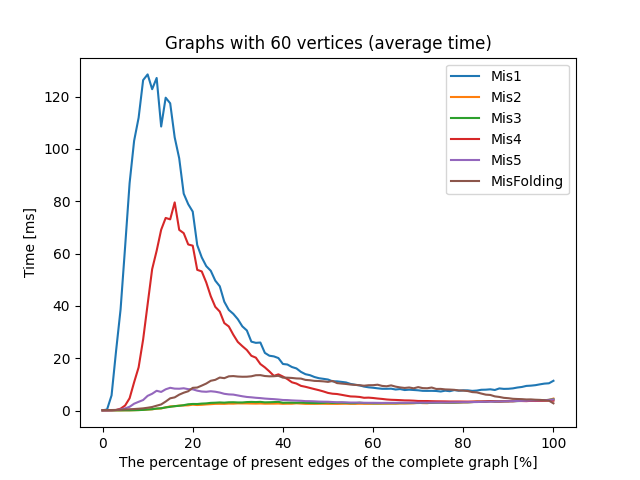
\includegraphics[width=\textwidth]{4_benchmark/plots/edges.png}
\centering
\end{figure}

\begin{figure}[H]
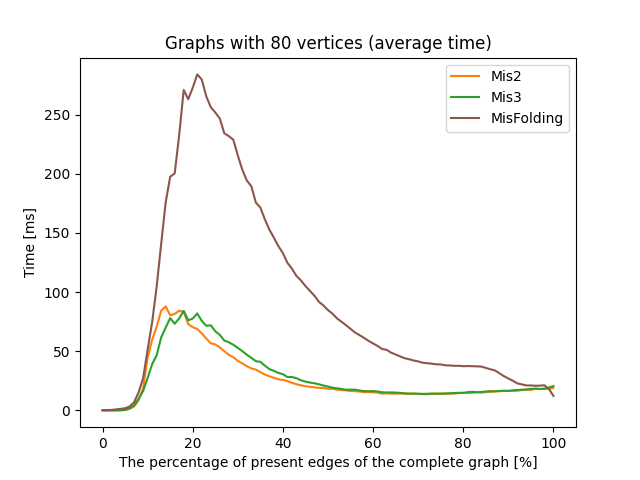
\includegraphics[width=\textwidth]{4_benchmark/plots/edges2.png}
\centering
\end{figure}


From the benchmarks performed, we can see that \textsc{MisNaive} is the slowest already for graphs as small as 10 vertices.

\textsc{Mis2} and \textsc{Mis3} are almost always the fastest for graphs up to about 100 vertices. \textsc{Mis3} algorithm is much simpler than \textsc{Mis2} but it offers a similar performance. To have a high-performance algorithm for graphs of these sizes (without much hassle) it is probably best to implement \textsc{Mis3} algorithm as well as data structures from scratch. NetworKit library has its limitations because it has to work well for all purposes. It does not perform well when graphs are heavily modified and recursion in our algorithms removes all vertices and edges.

As for graphs of higher sizes, we can see that \textsc{MisFolding} slowly gains an edge over \textsc{Mis2} and \textsc{Mis3}, at least in some specific cases. Unfortunately, we were not able to test it for graphs with larger order due to the long computing time.
